\documentclass[conference]{IEEEtran}

\usepackage[utf8]{inputenc}
\usepackage[T1]{fontenc}
\usepackage[brazilian]{babel}
\usepackage{graphicx}
\usepackage{booktabs}
\usepackage{cite}
\usepackage{url}

\begin{document}

\title{Reconhecimento de Atividades Humanas com Sensores de Movimento de Smartphone: Comparação entre SVM e Random Forest em Participantes Não Vistos no Treino}

% Substituir pelos nomes reais do grupo.
\author{
  \IEEEauthorblockN{Autor 1, Autor 2, Autor 3, Autor 4}
  \IEEEauthorblockA{Curso de Graduação, Instituição\\
  \texttt{email@instituicao.br}}
}

\maketitle

\begin{abstract}
% Escrever por último, com resultados reais: problema, método, resultados e conclusão.
\end{abstract}

\begin{IEEEkeywords}
reconhecimento de atividades humanas, sensores inerciais, SVM, Random Forest, validação por participante
\end{IEEEkeywords}

% Responsável: Dev 1
\section{Introdução}

Smartphones modernos trazem acelerômetro e giroscópio, sensores que registram aceleração e rotação do aparelho. Essas medidas não dizem diretamente o que a pessoa está fazendo, mas variam de forma característica conforme a atividade: caminhar, subir escadas, ficar sentado ou deitado produzem padrões de movimento distintos. Reconhecer atividades a partir desses sinais permite aplicações como monitoramento de saúde, acompanhamento de idosos e estímulo à atividade física, sem exigir equipamento além do telefone.

Um modelo desse tipo só é útil se funcionar para pessoas que não participaram do seu treinamento. Quando janelas consecutivas de uma mesma pessoa aparecem no treino e na avaliação, o resultado tende a ser otimista, pois o modelo pode aprender traços individuais em vez da atividade. Por isso, este trabalho avalia os modelos com participantes inteiros separados entre treino e validação.

Este trabalho compara duas técnicas de aprendizado de máquina, Máquinas de Vetores de Suporte (SVM) e Random Forest, no reconhecimento de seis atividades cotidianas a partir de um smartphone preso à cintura. Os dados são do conjunto UCI HAR \cite{anguita2013,uci_har}. As perguntas de pesquisa são:

\begin{enumerate}
  \item Com que precisão as seis atividades são reconhecidas para participantes não vistos no treino?
  \item Como SVM e Random Forest se comparam em desempenho de reconhecimento e custo computacional?
  \item Quais atividades são mais confundidas e quais características dos sensores ajudam a distingui-las?
\end{enumerate}

O restante do artigo está organizado da seguinte forma. A Seção~II revisa trabalhos relacionados. A Seção~III descreve o conjunto de dados e a metodologia. A Seção~IV apresenta os modelos, a Seção~V os resultados, a Seção~VI a discussão e a Seção~VII a conclusão.

% Responsável: todos (cada integrante traz 1 a 2 artigos).
% Ponto de partida: o estudo original do conjunto de dados \cite{anguita2013}.
\section{Trabalhos Relacionados}

\section{Conjunto de Dados e Metodologia}

% Responsável pelo Dataset: Dev 1
\subsection{Conjunto de dados}

Foi usado o conjunto \emph{Human Activity Recognition Using Smartphones} \cite{anguita2013,uci_har}. Trinta voluntários, entre 19 e 48 anos, realizaram seis atividades carregando um smartphone preso à cintura: caminhar, subir escadas, descer escadas, sentar, ficar em pé e deitar. O acelerômetro e o giroscópio foram amostrados a 50~Hz, e os sinais foram divididos em janelas de 2,56~s com 50\% de sobreposição. Os dados são medidas numéricas dos sensores; os vídeos foram usados pelos autores originais apenas para anotar as atividades.

Cada janela é descrita por 561 características calculadas nos domínios do tempo e da frequência, normalizadas para o intervalo $[-1, 1]$. O conjunto totaliza 10.299 janelas e traz a divisão oficial em treino, com 7.352 janelas de 21 participantes, e teste, com 2.947 janelas de 9 participantes diferentes. Essa divisão foi mantida. A identificação do participante é usada somente para separar e validar os dados, nunca como entrada dos modelos.

A análise exploratória (Tabela~\ref{tab:splits} e Figura~\ref{fig:classes}) mostrou que as classes são razoavelmente equilibradas, entre 13\% e 19\% das janelas, e que todos os participantes têm exemplos das seis atividades, com 281 a 409 janelas cada. Não há valores ausentes, linhas repetidas nem características constantes.

\begin{table}[t]
  \caption{Divisão oficial do conjunto de dados.}
  \label{tab:splits}
  \centering
  \begin{tabular}{lrrr}
    \toprule
    Partição & Janelas & Participantes & Características \\
    \midrule
    Treino & 7.352 & 21 & 561 \\
    Teste  & 2.947 & 9  & 561 \\
    \bottomrule
  \end{tabular}
\end{table}

\begin{figure}[t]
  \centering
  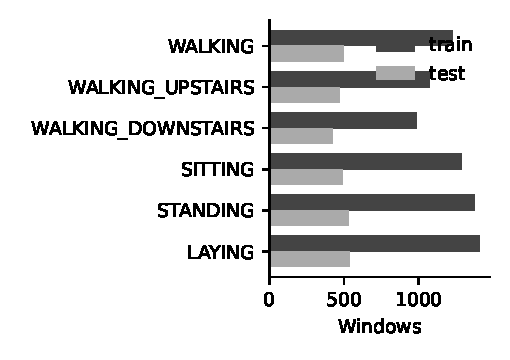
\includegraphics[width=\columnwidth]{figures/class_distribution.pdf}
  \caption{Janelas por atividade nas partições de treino e teste.}
  \label{fig:classes}
\end{figure}

% Responsável pela Metodologia: Dev 2 (validação agrupada, métricas, semente e versões).
\subsection{Metodologia}

% Responsáveis: Dev 3 (SVM e hiperparâmetros) e Dev 4 (Random Forest e hiperparâmetros).
\section{Modelos}

% Escrever somente depois dos experimentos. Os números devem vir de results/metrics/*.json.
% Dev 2: tabela comparativa. Dev 3: matrizes de confusão. Dev 4: importância de características.
\section{Resultados}

% Responsável: Dev 2, com todos. Interpretação, generalização, custo computacional e limitações.
\section{Discussão e Limitações}

% Responsável: todos. Responder às três perguntas de pesquisa e indicar trabalhos futuros.
\section{Conclusão}


\bibliographystyle{IEEEtran}
\bibliography{refs}

\end{document}
